\documentclass[../../main]{subfiles}

\renewcommand\thesection{\arabic{section}}


\begin{document}

\section{Air Moisture Control System} \label{sec:}

The \emph{air moisture control system} make use of \emph{piezoelectric} humidifiers.
As they are placed in water and powered, they can vibrate in the \emph{ultrasonic} ranges,
and sprays water as particles into the air.

\alertNote{
    These humidifiers can only increase the humidity of the atmosphere, in order to decrease
    the relative humidity, they need to work with the \emph{exhaust system} mentioned in the
    section \ref{sec:thermalControlAndExhaustSystem}.
}

\subsection{Piezoelectric Humidifiers}

\begin{center}
    {\begin{minipage} [c] {0.55\textwidth}

        These \emph{piezoelectric} humidifiers have two parts, one is the \emph{piezoelectric disc}
        itself and the other is the driving circuit. These \emph{discs} have a \emph{resonant}
        frequency. And we need to drive them in this specific frequency to get the maximum output.
        Figure \ref{fig:piezoHumidifierImage} shows the module.

        Specification:

        \begin{itemize}
            \item \textbf{Operating voltage:} $4.5\si{V}$ to $5\si{V}$.
            \item \textbf{Resonant frequency:} $108\si{kHz} \pm 3\si{kHz}$.
            \item \textbf{Spray quantitiy:} $380 \si{mL/h}$.
            \item \textbf{Work power:} $2\si{W}$.
        \end{itemize}

    \end{minipage}
    \hfill
    \begin{minipage} [c] {0.35\textwidth}
        \centering
        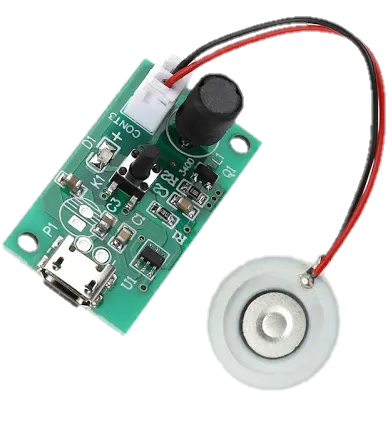
\includegraphics [
            max width = \IGXMaxWidth,
            max height = \IGXMaxHeight,
            \IGXDefaultOptionalArgs,
        ] {pics/humidifier.png}
        \captionof{figure} {
            Piezoelectric humidifier module.
            \label{fig:piezoHumidifierImage}
        }
    \end{minipage}\hfill}
\end{center}

\subsection{Interfacing}

The driver module is just a $555$ timer circuit. And if we look closely at figure \ref{fig:piezoHumidifierImage}
we can see a push button. If we press once\footnote{given that the module is powered and in off state.}, the
module will turn on. And if we press twice\footnote{given that the module was already on.}, the module will
turn off. If we \emph{trace} the PCB \emph{tracing}, we can see that the push button is simply connecting the
some of the pins to ground, when it is being pressed.

With that information we can now turn on and turn off the module using one of the GPIOs of \esp. We simply
keep the pin high and keep the \emph{state} of the humidifier \emph{internally}\footnote{as in some variable.}.
When we want to turn on the module, we can simply give a \emph{low pulse} using this pin. And if we want
to turn off the module, we can simply give two pulses.

Refer figure \ref{fig:absHumidifierSystem} for the interfacing of the module, with \esp.

\begin{figure}
    \centering
    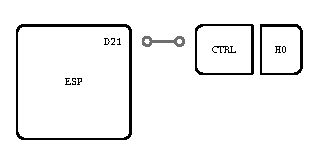
\includegraphics [
        max width = \IGXMaxWidth,
        max height = \IGXMaxHeight,
        \IGXDefaultOptionalArgs,
    ] {tikzpics/endAbsHumidifierSystem.pdf}
    \captionof{figure} {Interfacing of piezoelectric humidifier module.}
    \label{fig:absHumidifierSystem}
\end{figure}

\alertNote{
    Trigger pin of \emph{humidifier} is connected to the \texttt{D21} of the \esp as we can see
    from figure \ref{fig:absHumidifierSystem}.
}

\alertImportant{
    Right now, the \emph{humidifier} is triggered directly from the \esp itself. In the future
    all the \emph{actuator control} will be moved to the \emph{auxiliary system} with a separate
    control board\footnote{will be another shift register board.} and \esp will simply interface
    the board through couple of pins.
}

\end{document}
